\chapter{Dérivabilité et Étude des Fonctions}

Ce chapitre approfondit l'étude locale et globale des fonctions d'une variable réelle. Nous allons compléter l'étude de la dérivation (fonction composée, réciproque), introduire les théorèmes fondamentaux de l'analyse réelle (Rolle, Accroissements Finis) et détailler la caractérisation géométrique des courbes (branches infinies, concavité).

\section{Compléments sur la Dérivation}

\subsection{Dérivée d'une fonction composée}

\begin{theoreme}[Dérivée de $v \circ u$]
Soit $u$ une fonction dérivable sur un intervalle $I$ à valeurs dans un intervalle $J$, et $v$ une fonction dérivable sur $J$.
La fonction composée $f = v \circ u$ définie sur $I$ par $f(x) = v(u(x))$ est dérivable sur $I$, et pour tout $x \in I$ :
\[
f'(x) = v'(u(x)) \times u'(x)
\]
\end{theoreme}

De ce théorème général découlent plusieurs formules clés à connaître sur le bout des doigts :

\begin{propriete}[Cas particuliers usuels]
Soit $u$ une fonction dérivable sur un intervalle $I$.
\begin{itemize}
    \item \textbf{Puissance} : La fonction $u^n$ ($n \in \N^*$) est dérivable sur $I$ et de dérivée :
    \[
    (u^n)' = n u^{n-1} u'
    \]
    \item \textbf{Racine} : Si pour tout $x \in I$, $u(x) > 0$, la fonction $\sqrt{u}$ est dérivable sur $I$ et de dérivée :
    \[
    (\sqrt{u})' = \frac{u'}{2\sqrt{u}}
    \]
    \item \textbf{Exponentielle} : La fonction $e^u$ est dérivable sur $I$ et de dérivée :
    \[
    (e^u)' = u' e^u
    \]
\end{itemize}
\end{propriete}

\subsection{Dérivée seconde}

\begin{definition}[Dérivées successives]
Soit $f$ une fonction dérivable sur un intervalle $I$. Si la fonction dérivée $f'$ est elle-même dérivable sur $I$, sa dérivée, notée $f''$, est appelée la \textbf{dérivée seconde} de $f$.
\end{definition}

\subsection{Dérivabilité de la fonction réciproque}

\begin{theoreme}[Dérivabilité de $f^{-1}$]
Soit $f$ une fonction continue et strictement monotone sur un intervalle $I$. Soit $J = f(I)$ l'intervalle image.
Si $f$ est dérivable en un point $x_0 \in I$ et si $f'(x_0) \ne 0$, alors sa fonction réciproque $f^{-1}$ est dérivable en $y_0 = f(x_0) \in J$, et :
\[
(f^{-1})'(y_0) = \frac{1}{f'(x_0)} = \frac{1}{f'(f^{-1}(y_0))}
\]
Si $f$ est dérivable sur $I$ et si sa dérivée $f'$ ne s'annule pas sur $I$, alors $f^{-1}$ est dérivable sur $J$, et pour tout $y \in J$ :
\[
(f^{-1})'(y) = \frac{1}{f'(f^{-1}(y))}
\]
\end{theoreme}

\begin{propriete}[Dérivées de la racine $n$-ième et de l'arctangente]
\begin{itemize}
    \item La fonction racine $n$-ième ($x \mapsto \sqrt[n]{x}$) est dérivable sur $]0, +\infty[$ et :
    \[
    (\sqrt[n]{x})' = \frac{1}{n\sqrt[n]{x^{n-1}}} = \frac{1}{n} x^{\frac{1}{n}-1}
    \]
    Note : elle n'est pas dérivable à droite en 0, sa courbe admet une demi-tangente verticale à l'origine.
    \item La fonction Arctangente ($x \mapsto \arctan(x)$) est dérivable sur $\R$ et :
    \[
    (\arctan(x))' = \frac{1}{1+x^2}
    \]
\end{itemize}
\end{propriete}

\section{Théorèmes Fondamentaux (Rolle et Accroissements Finis)}

Ces deux théorèmes fournissent des liens puissants entre le comportement d'une fonction et les valeurs de sa dérivée.

\subsection{Théorème de Rolle}

\begin{theoreme}[Théorème de Rolle]
Soit $f$ une fonction réelle continue sur $[a, b]$ et dérivable sur $]a, b[$.
Si $f(a) = f(b)$, alors il existe au moins un réel $c \in ]a, b[$ tel que :
\[
f'(c) = 0
\]
\end{theoreme}

Géométriquement, cela signifie que si les extrémités d'une courbe continue et lisse ont la même ordonnée, alors il existe au moins un point de la courbe où la tangente est horizontale.

\subsection{Théorème des Accroissements Finis (TAF)}

\begin{theoreme}[Théorème des Accroissements Finis]
Soit $f$ une fonction réelle continue sur $[a, b]$ et dérivable sur $]a, b[$.
Alors il existe au moins un réel $c \in ]a, b[$ tel que :
\[
f(b) - f(a) = f'(c)(b-a)
\]
\end{theoreme}

Géométriquement, cela signifie qu'il existe un point $c \in ]a,b[$ où la tangente à la courbe est parallèle à la sécante reliant les points de coordonnées $(a, f(a))$ et $(b, f(b))$.

\begin{theoreme}[Inégalité des Accroissements Finis (IAF)]
Soit $f$ une fonction continue sur un intervalle $I$ et dérivable sur l'intérieur de $I$.
S'il existe deux réels $m$ et $M$ tels que pour tout $x$ intérieur à $I$, $m \le f'(x) \le M$, alors pour tous réels $a$ et $b$ de $I$ avec $a \le b$ :
\[
m(b-a) \le f(b) - f(a) \le M(b-a)
\]
En particulier, s'il existe une constante $k \ge 0$ telle que pour tout $x \in I$, $|f'(x)| \le k$, alors :
\[
|f(b) - f(a)| \le k |b-a|
\]
\end{theoreme}

\section{Branches Infinies et Étude des Fonctions}

L'étude des branches infinies permet de décrire le comportement asymptotique des courbes représentatives $\mathcal{C}_f$ de fonctions au voisinage de $\pm\infty$ ou de points de discontinuité.

\subsection{Asymptotes}
\begin{itemize}
    \item \textbf{Asymptote verticale} : Si $\lim_{x \to a} f(x) = \pm\infty$, la droite d'équation $x = a$ est une asymptote verticale à la courbe $\mathcal{C}_f$.
    \item \textbf{Asymptote horizontale} : Si $\lim_{x \to \pm\infty} f(x) = L$ ($L \in \R$), la droite d'équation $y = L$ est une asymptote horizontale à la courbe $\mathcal{C}_f$ en $\pm\infty$.
    \item \textbf{Asymptote oblique} : Si $\lim_{x \to \pm\infty} [f(x) - (ax+b)] = 0$ ($a \ne 0$), la droite d'équation $y = ax+b$ est une asymptote oblique à la courbe $\mathcal{C}_f$ en $\pm\infty$.
\end{itemize}

\subsection{Branches paraboliques}
Si $\lim_{x \to \pm\infty} f(x) = \pm\infty$, on étudie la limite du rapport $\frac{f(x)}{x}$ :
\begin{itemize}
    \item \textbf{Direction l'axe $(Oy)$} : Si $\lim_{x \to \pm\infty} \frac{f(x)}{x} = \pm\infty$, la courbe $\mathcal{C}_f$ admet une \textbf{branche parabolique de direction l'axe des ordonnées $(Oy)$}.
    \item \textbf{Direction l'axe $(Ox)$} : Si $\lim_{x \to \pm\infty} \frac{f(x)}{x} = 0$, la courbe $\mathcal{C}_f$ admet une \textbf{branche parabolique de direction l'axe des abscisses $(Ox)$}.
    \item \textbf{Direction la droite $y = ax$} : Si $\lim_{x \to \pm\infty} \frac{f(x)}{x} = a \ne 0$, on étudie alors la limite de la différence $f(x) - ax$ :
    \begin{itemize}
        \item Si $\lim_{x \to \pm\infty} [f(x) - ax] = \pm\infty$, la courbe $\mathcal{C}_f$ admet une \textbf{branche parabolique de direction la droite d'équation $y = ax$}.
        \item Si $\lim_{x \to \pm\infty} [f(x) - ax] = b$, alors la droite d'équation $y = ax+b$ est une asymptote oblique.
    \end{itemize}
\end{itemize}

\section{Concavité d'une courbe et Points d'Inflexion}

L'étude de la concavité permet de déterminer la direction de la courbure de la courbe représentative $\mathcal{C}_f$ d'une fonction et d'identifier les points de transition appelés points d'inflexion.

\subsection{Concavité d'une courbe}

\begin{definition}[Courbe convexe et courbe concave]
Soit $f$ une fonction dérivable sur un intervalle $I$ et $\mathcal{C}_f$ sa courbe représentative.
\begin{itemize}
    \item On dit que la courbe $\mathcal{C}_f$ est \textbf{convexe} sur $I$ si elle est située entièrement au-dessus de toutes ses tangentes sur $I$.
    \item On dit que la courbe $\mathcal{C}_f$ est \textbf{concave} sur $I$ si elle est située entièrement au-dessous de toutes ses tangentes sur $I$.
\end{itemize}
\end{definition}

\subsection{Caractérisation par la dérivée seconde}

\begin{theoreme}[Caractérisation de la concavité]
Soit $f$ une fonction deux fois dérivable sur un intervalle $I$.
\begin{itemize}
    \item La courbe $\mathcal{C}_f$ est convexe sur $I$ si et seulement si pour tout $x \in I$, $f''(x) \ge 0$.
    \item La courbe $\mathcal{C}_f$ est concave sur $I$ si et seulement si pour tout $x \in I$, $f''(x) \le 0$.
\end{itemize}
\end{theoreme}

\subsection{Point d'inflexion}

\begin{definition}[Point d'inflexion]
Soit $f$ une fonction dérivable sur un intervalle $I$.
Un point $A(a, f(a))$ est appelé un \textbf{point d'inflexion} de la courbe $\mathcal{C}_f$ si la courbe change de concavité en $a$. Géométriquement, la courbe traverse sa tangente au point $A$.
\end{definition}

\begin{theoreme}[Caractérisation analytique du point d'inflexion]
Soit $f$ une fonction deux fois dérivable sur un intervalle $I$.
Le point $A(a, f(a))$ est un point d'inflexion de $\mathcal{C}_f$ si et seulement si la dérivée seconde $f''$ \textbf{s'annule en changeant de signe} en $a$.
\end{theoreme}

Voici une illustration avec la courbe de $f(x) = x^3 - 3x^2 + 2$ qui change de concavité au point d'inflexion $I(1,0)$ :

\begin{center}
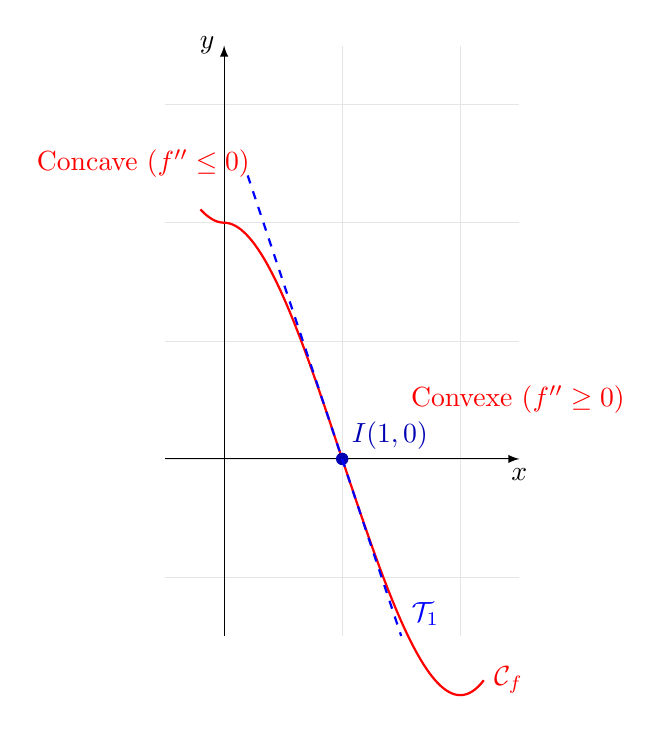
\begin{tikzpicture}[scale=1.5]
  % Grille de fond
  \draw[gray!20,very thin] (-0.5,-1.5) grid (2.5,3.5);
  % Axes
  \draw[->,>=latex] (-0.5,0) -- (2.5,0) node[below] {$x$};
  \draw[->,>=latex] (0,-1.5) -- (0,3.5) node[left] {$y$};
  
  % Courbe représentative de f
  \draw[domain=-0.2:2.2, samples=100, color=red, thick] plot (\x, {\x^3 - 3*\x^2 + 2}) node[right] {$\mathcal{C}_f$};
  
  % Point d'inflexion
  \fill[blue!70!black] (1,0) circle (1.5pt) node[above right] {$I(1,0)$};
  
  % Tangente d'inflexion en x=1 : y = -3x + 3
  \draw[domain=0.2:1.5, color=blue, thick, dashed] plot (\x, {-3*\x + 3}) node[above right] {$\mathcal{T}_1$};
  
  % Textes explicatifs
  \node[left, red] at (0.3, 2.5) {Concave ($f'' \le 0$)};
  \node[right, red] at (1.5, 0.5) {Convexe ($f'' \ge 0$)};
\end{tikzpicture}
\end{center}

\section{Méthodes Clés}

\begin{methode}[Étudier la concavité et les points d'inflexion]
Pour déterminer la concavité de la courbe $\mathcal{C}_f$ et ses éventuels points d'inflexion :
\begin{enumerate}
    \item On calcule la dérivée première $f'(x)$.
    \item On calcule la dérivée seconde $f''(x)$.
    \item On étudie le signe de $f''(x)$ sur l'ensemble de définition :
    \begin{itemize}
        \item Sur les intervalles où $f''(x) \ge 0$, la courbe $\mathcal{C}_f$ est convexe (courbée vers le haut).
        \item Sur les intervalles où $f''(x) \le 0$, la courbe $\mathcal{C}_f$ est concave (courbée vers le bas).
        \item Les points où $f''(x)$ s'annule en changeant de signe sont des points d'inflexion.
    \end{itemize}
\end{enumerate}
\end{methode}

\begin{exemple}[Étude de la concavité]
Soit la fonction $f$ définie sur $\R$ par $f(x) = (x^2-2x)e^x$.
Calculons les dérivées successives :
\[
f'(x) = (2x-2)e^x + (x^2-2x)e^x = (x^2-2)e^x
\]
Puis la dérivée seconde :
\[
f''(x) = (2x)e^x + (x^2-2)e^x = (x^2+2x-2)e^x
\]
Comme $e^x > 0$, le signe de $f''(x)$ est celui du polynôme $x^2+2x-2$. Le discriminant est $\Delta = 12 > 0$. Les racines sont :
\[
x_1 = -1-\sqrt{3} \approx -2,73 \quad \text{et} \quad x_2 = -1+\sqrt{3} \approx 0,73
\]
Ainsi :
\begin{itemize}
    \item la courbe $\mathcal{C}_f$ est convexe sur $]-\infty, -1-\sqrt{3}]$ et sur $[-1+\sqrt{3}, +\infty[$.
    \item la courbe $\mathcal{C}_f$ est concave sur $[-1-\sqrt{3}, -1+\sqrt{3}]$.
    \item La courbe $\mathcal{C}_f$ admet deux points d'inflexion aux abscisses $x_1$ et $x_2$.
\end{itemize}
\end{exemple}

\section{Exercices d'Entraînement Résolus}

\subsection*{Exercice 1 : Dérivée d'une puissance de fonction}
Déterminer la dérivée de la fonction $f$ définie sur $\R$ par :
\[
f(x) = (3x^2 + 1)^5
\]

\textbf{Solution :}
La fonction $f$ est de la forme $u^n$ avec $u(x) = 3x^2 + 1$ et $n = 5$.
La fonction $u$ est dérivable sur $\R$ et $u'(x) = 6x$.
D'après la formule $(u^n)' = n u^{n-1} u'$, on a :
\[
f'(x) = 5(3x^2 + 1)^4 \times 6x = 30x(3x^2 + 1)^4
\]

\subsection*{Exercice 2 : Dérivée d'une racine de fonction}
Déterminer la dérivée de la fonction $f$ définie sur $\R$ par :
\[
f(x) = \sqrt{e^x + x^2 + 1}
\]

\textbf{Solution :}
La fonction $f$ est de la forme $\sqrt{u}$ avec $u(x) = e^x + x^2 + 1$.
Puisque $e^x > 0$, $x^2 \ge 0$ et $1 > 0$, on a $u(x) > 0$ pour tout $x \in \R$.
La fonction $u$ est dérivable sur $\R$ et $u'(x) = e^x + 2x$.
D'après la formule $(\sqrt{u})' = \frac{u'}{2\sqrt{u}}$, on a :
\[
f'(x) = \frac{e^x + 2x}{2\sqrt{e^x + x^2 + 1}}
\]

\subsection*{Exercice 3 : Dérivée de l'exponentielle d'une fonction}
Déterminer la dérivée de la fonction $f$ définie sur $\R$ par :
\[
f(x) = e^{2x^2 - 3x}
\]

\textbf{Solution :}
La fonction $f$ est de la forme $e^u$ avec $u(x) = 2x^2 - 3x$.
La fonction $u$ est dérivable sur $\R$ et $u'(x) = 4x - 3$.
D'après la formule $(e^u)' = u' e^u$, on a :
\[
f'(x) = (4x - 3)e^{2x^2 - 3x}
\]

\subsection*{Exercice 4 : Dérivée du logarithme d'une fonction}
Déterminer la dérivée de la fonction $f$ définie sur $\R$ par :
\[
f(x) = \ln(x^2 + 1)
\]

\textbf{Solution :}
La fonction $f$ est de la forme $\ln(u)$ avec $u(x) = x^2 + 1$.
Pour tout $x \in \R$, $x^2 + 1 \ge 1 > 0$. $f$ est donc bien définie et dérivable sur $\R$.
La fonction $u$ est dérivable et $u'(x) = 2x$.
D'après la formule $(\ln(u))' = \frac{u'}{u}$, on a :
\[
f'(x) = \frac{2x}{x^2 + 1}
\]

\subsection*{Exercice 5 : Calcul de dérivée seconde}
Déterminer la dérivée seconde de la fonction $f$ définie sur $\R$ par :
\[
f(x) = x e^x
\]

\textbf{Solution :}
La fonction $f$ est de la forme $uv$ avec $u(x) = x$ et $v(x) = e^x$.
- Dérivée première :
  \[
  f'(x) = u'(x)v(x) + u(x)v'(x) = 1 \cdot e^x + x \cdot e^x = (x+1)e^x
  \]
- Dérivée seconde (en dérivant $f'(x)$ qui est de la forme $g(x)e^x$ avec $g(x) = x+1$ et $g'(x) = 1$) :
  \[
  f''(x) = g'(x)e^x + g(x)e^x = 1 \cdot e^x + (x+1)e^x = (x+2)e^x
  \]

\subsection*{Exercice 6 : Détermination des intervalles de convexité}
Étudier la convexité de la fonction $f$ définie sur $\R$ par $f(x) = 2x^3 - 9x^2 + 12x$.

\textbf{Solution :}
La fonction $f$ est polynomiale donc deux fois dérivable sur $\R$.
- $f'(x) = 6x^2 - 18x + 12$
- $f''(x) = 12x - 18 = 6(2x - 3)$
Étudions le signe de $f''(x)$ :
\[
f''(x) \ge 0 \iff 2x - 3 \ge 0 \iff x \ge \frac{3}{2}
\]
Ainsi :
\begin{itemize}
    \item $f$ est **concave** sur l'intervalle $\left]-\infty, \frac{3}{2}\right]$ car $f''(x) \le 0$.
    \item $f$ est **convexe** sur l'intervalle $\left[\frac{3}{2}, +\infty\right[$ car $f''(x) \ge 0$.
\end{itemize}

\subsection*{Exercice 7 : Recherche de points d'inflexion}
Déterminer les coordonnées des points d'inflexion de la courbe représentative de la fonction $f$ définie sur $\R$ par :
\[
f(x) = x^4 - 6x^2
\]

\textbf{Solution :}
La fonction $f$ est deux fois dérivable sur $\R$.
- $f'(x) = 4x^3 - 12x$
- $f''(x) = 12x^2 - 12 = 12(x^2 - 1) = 12(x-1)(x+1)$
La dérivée seconde $f''$ s'annule pour $x = -1$ et $x = 1$. Le coefficient devant $x^2$ étant positif ($12>0$), $f''(x)$ change de signe en passant par ces racines (elle est positive à l'extérieur, négative à l'intérieur).
La courbe $\mathcal{C}_f$ admet donc deux points d'inflexion :
- Pour $x = -1$ : $f(-1) = (-1)^4 - 6(-1)^2 = 1 - 6 = -5$. Le point est $I_1(-1, -5)$.
- Pour $x = 1$ : $f(1) = 1^4 - 6(1)^2 = -5$. Le point est $I_2(1, -5)$.

\subsection*{Exercice 8 : Démonstration d'inégalité par convexité}
Démontrer que la fonction exponentielle est convexe sur $\R$, et en déduire que pour tout $x \in \R$ :
\[
e^x \ge x + 1
\]

\textbf{Solution :}
Soit $f(x) = e^x$. La fonction $f$ est deux fois dérivable sur $\R$ et pour tout $x \in \R$, $f''(x) = e^x > 0$.
La fonction exponentielle est donc strictement convexe sur $\R$.
Par définition, sa courbe représentative $\mathcal{C}_f$ est située au-dessus de toutes ses tangentes.
Déterminons l'équation de la tangente $\mathcal{T}_0$ à la courbe en $x=0$ :
\[
y = f'(0)(x-0) + f(0) \implies y = e^0 x + e^0 \implies y = x + 1
\]
La courbe étant située au-dessus de sa tangente en 0, on a pour tout $x \in \R$ :
\[
e^x \ge x + 1
\]

\subsection*{Exercice 9 : Convexité d'une fonction avec logarithme}
Soit la fonction $f$ définie sur $]0, +\infty[$ par $f(x) = x \ln(x)$. Étudier la convexité de $f$.

\textbf{Solution :}
La fonction $f$ est dérivable sur $]0, +\infty[$.
- Dérivée première : $f'(x) = 1 \cdot \ln(x) + x \cdot \frac{1}{x} = \ln(x) + 1$.
- Dérivée seconde : $f''(x) = \frac{1}{x}$.
Pour tout $x \in ]0, +\infty[$, $f''(x) = \frac{1}{x} > 0$.
Puisque sa dérivée seconde est strictement positive sur son ensemble de définition, la fonction $f$ est **strictement convexe** sur $]0, +\infty[$.

\subsection*{Exercice 10 : Dérivée de l'inverse d'une fonction}
Soit $u$ une fonction dérivable et strictement positive sur un intervalle $I$. Soit $f = \frac{1}{u}$.
Rappeler la formule de la dérivée de $f$, et en déduire son sens de variation si $u$ est strictement croissante sur $I$.

\textbf{Solution :}
La fonction $f = \frac{1}{u}$ est dérivable sur $I$ et de dérivée :
\[
f'(x) = -\frac{u'(x)}{u(x)^2}
\]
Si $u$ est strictement croissante sur $I$, alors pour tout $x \in I$, $u'(x) > 0$.
De plus, $u(x)^2 > 0$ car $u$ est strictement positive.
Ainsi, le quotient $\frac{u'(x)}{u(x)^2}$ est strictement positif, et son opposé $f'(x) = -\frac{u'(x)}{u(x)^2}$ est strictement négatif.
On en déduit que la fonction $f = \frac{1}{u}$ est **strictement décroissante** sur $I$.

\subsection*{Exercice 11 : Dérivée d'une fonction composée avec Arctangente}
Soit la fonction $f$ définie sur $\R$ par $f(x) = \arctan(e^x)$. Montrer que $f$ est dérivable sur $\R$ et calculer sa dérivée.

\textbf{Solution :}
La fonction $f$ est la composée de $u(x) = e^x$ et de $v(y) = \arctan(y)$.
- La fonction $u$ est dérivable sur $\R$ et pour tout $x \in \R$, $u'(x) = e^x$.
- La fonction $v$ est dérivable sur $\R$ et pour tout $y \in \R$, $v'(y) = \frac{1}{1+y^2}$.
D'après la formule de dérivation d'une fonction composée $(v \circ u)' = (v' \circ u) \times u'$, la fonction $f$ est dérivable sur $\R$ et :
\[
f'(x) = \frac{1}{1+(e^x)^2} \times e^x = \frac{e^x}{1+e^{2x}}
\]

\subsection*{Exercice 12 : Application du Théorème des Accroissements Finis}
Démontrer que pour tous réels $a$ et $b$ tels que $0 \le a < b$ :
\[
\frac{b-a}{1+b^2} < \arctan(b) - \arctan(a) < \frac{b-a}{1+a^2}
\]

\textbf{Solution :}
Soit la fonction $g(x) = \arctan(x)$. La fonction $g$ est continue sur $[a, b]$ et dérivable sur $]a, b[$.
D'après le Théorème des Accroissements Finis (TAF), il existe un réel $c \in ]a, b[$ tel que :
\[
g(b) - g(a) = g'(c)(b-a) \implies \arctan(b) - \arctan(a) = \frac{b-a}{1+c^2}
\]
Puisque $0 \le a < c < b$, en élevant au carré et en ajoutant 1 (les termes étant positifs) :
\[
a^2 < c^2 < b^2 \implies 1+a^2 < 1+c^2 < 1+b^2 \implies \frac{1}{1+b^2} < \frac{1}{1+c^2} < \frac{1}{1+a^2}
\]
Comme $b-a > 0$, en multipliant par $b-a$, on obtient :
\[
\frac{b-a}{1+b^2} < \frac{b-a}{1+c^2} < \frac{b-a}{1+a^2}
\]
En remplaçant $\frac{b-a}{1+c^2}$ par sa valeur, on a bien :
\[
\frac{b-a}{1+b^2} < \arctan(b) - \arctan(a) < \frac{b-a}{1+a^2}
\]

\subsection*{Exercice 13 : Détermination d'une branche parabolique}
Soit la fonction $f$ définie sur $[0, +\infty[$ par $f(x) = x + \sqrt{x}$. Déterminer la nature de la branche infinie en $+\infty$.

\textbf{Solution :}
1. Calculons d'abord la limite en $+\infty$ :
   \[
   \lim_{x \to +\infty} f(x) = \lim_{x \to +\infty} (x + \sqrt{x}) = +\infty
   \]
2. Étudions le comportement de $\frac{f(x)}{x}$ en $+\infty$ :
   \[
   \frac{f(x)}{x} = \frac{x + \sqrt{x}}{x} = 1 + \frac{\sqrt{x}}{x} = 1 + \frac{1}{\sqrt{x}}
   \]
   Puisque $\lim_{x \to +\infty} \frac{1}{\sqrt{x}} = 0$, on a :
   \[
   a = \lim_{x \to +\infty} \frac{f(x)}{x} = 1
   \]
3. Le coefficient $a$ étant non nul, étudions la limite de la différence $f(x) - ax$ en $+\infty$ :
   \[
   f(x) - 1x = (x + \sqrt{x}) - x = \sqrt{x}
   \]
   Ainsi :
   \[
   \lim_{x \to +\infty} [f(x) - x] = \lim_{x \to +\infty} \sqrt{x} = +\infty
   \]
On en conclut que la courbe représentative $\mathcal{C}_f$ admet une **branche parabolique de direction la droite d'équation $y = x$** en $+\infty$.

\section{Problèmes Résolus}

\subsection*{Problème 1 : Optimisation de la surface d'une boîte de conserve}
On souhaite concevoir une boîte de conserve cylindrique fermée de volume fixé $V = 1 \text{ dm}^3$ ($1000 \text{ cm}^3$). On note $r$ le rayon de la base du cylindre (en cm) et $h$ sa hauteur (en cm).
\begin{enumerate}
    \item Exprimer le volume $V$ en fonction de $r$ et $h$. En déduire $h$ en fonction de $r$.
    \item Montrer que l'aire totale $S(r)$ de la boîte de conserve (les deux bases circulaires et la paroi latérale) est donnée par :
    \[
    S(r) = 2\pi r^2 + \frac{2000}{r}
    \]
    \item Étudier les variations de la fonction $S$ sur $]0, +\infty[$.
    \item En déduire le rayon $r_0$ (en cm) qui permet de minimiser la quantité de métal utilisée pour fabriquer cette boîte. Calculer alors la hauteur correspondante $h_0$ et montrer que $h_0 = 2r_0$.
\end{enumerate}

\textbf{Solution :}
\begin{enumerate}
    \item Le volume d'un cylindre est donné par : $V = \pi r^2 h$.
    Puisque $V = 1000$, on a $\pi r^2 h = 1000 \implies h = \frac{1000}{\pi r^2}$.
    
    \item L'aire totale est la somme de l'aire latérale et de l'aire des deux bases :
    \[
    S(r) = 2 \times (\pi r^2) + 2\pi r h = 2\pi r^2 + 2\pi r \left( \frac{1000}{\pi r^2} \right) = 2\pi r^2 + \frac{2000}{r}
    \]
    
    \item La fonction $S$ est dérivable sur $]0, +\infty[$ :
    \[
    S'(r) = 4\pi r - \frac{2000}{r^2} = \frac{4\pi r^3 - 2000}{r^2} = \frac{4(\pi r^3 - 500)}{r^2}
    \]
    Le dénominateur $r^2$ étant positif, le signe de $S'(r)$ est celui de $\pi r^3 - 500$.
    \[
    S'(r) \ge 0 \iff \pi r^3 - 500 \ge 0 \iff r^3 \ge \frac{500}{\pi} \iff r \ge \sqrt[3]{\frac{500}{\pi}} \approx 5,42 \text{ cm}
    \]
    La fonction $S$ est donc strictement décroissante sur $\left]0, \sqrt[3]{\frac{500}{\pi}}\right]$ et strictement croissante sur $\left[\sqrt[3]{\frac{500}{\pi}}, +\infty\right[$.
    
    \item L'aire est minimale pour le rayon :
    \[
    r_0 = \sqrt[3]{\frac{500}{\pi}} \approx 5,42 \text{ cm}
    \]
    Calculons la hauteur $h_0$ correspondante en utilisant $r_0^3 = \frac{500}{\pi}$ :
    \[
    h_0 = \frac{1000}{\pi r_0^2} = \frac{2 \times 500}{\pi r_0^2} = \frac{2 \times (\pi r_0^3)}{\pi r_0^2} = 2r_0
    \]
    La hauteur optimale est égale au diamètre du cylindre, ce qui donne une boîte bien proportionnée.
\end{enumerate}

\subsection*{Problème 2 : Recherche de tangentes communes}
On considère la courbe $\mathcal{C}_1$ associée à la fonction $f(x) = x^2$ et la courbe $\mathcal{C}_2$ associée à la fonction $g(x) = -x^2 + 2x - 3$.
Déterminer s'il existe une ou plusieurs droites tangentes simultanément à $\mathcal{C}_1$ et $\mathcal{C}_2$. Si oui, donner leurs équations.

\textbf{Solution :}
Soit $a$ l'abscisse du point de tangence sur $\mathcal{C}_1$ et $b$ l'abscisse du point de tangence sur $\mathcal{C}_2$.
- L'équation de la tangente $\mathcal{T}_a$ à $\mathcal{C}_1$ en $a$ est (avec $f'(x) = 2x$) :
  \[
  y = f'(a)(x-a) + f(a) \implies y = 2ax - 2a^2 + a^2 \implies y = 2ax - a^2
  \]
- L'équation de la tangente $\mathcal{T}_b$ à $\mathcal{C}_2$ en $b$ est (avec $g'(x) = -2x+2$) :
  \[
  y = g'(b)(x-b) + g(b) \implies y = (-2b+2)(x-b) - b^2 + 2b - 3 \implies y = (2-2b)x + b^2 - 3
  \]
Les deux droites sont confondues si et seulement si leurs coefficients directeurs et leurs ordonnées à l'origine sont égaux, d'où le système :
\[
\begin{cases}
2a = 2 - 2b \\
-a^2 = b^2 - 3
\end{cases} \iff 
\begin{cases}
a = 1 - b \\
-(1 - b)^2 = b^2 - 3
\end{cases}
\]
En développant la seconde équation :
\[
-(1 - 2b + b^2) = b^2 - 3 \iff -1 + 2b - b^2 = b^2 - 3 \iff 2b^2 - 2b - 2 = 0 \iff b^2 - b - 1 = 0
\]
Le discriminant est $\Delta = (-1)^2 - 4(1)(-1) = 5 > 0$.
Les solutions pour $b$ sont $b_1 = \frac{1-\sqrt{5}}{2}$ et $b_2 = \frac{1+\sqrt{5}}{2}$.
- Si $b = b_1 = \frac{1-\sqrt{5}}{2}$, alors le coefficient directeur est $m_1 = 2-2b_1 = 1+\sqrt{5}$, et $a_1 = 1-b_1 = \frac{1+\sqrt{5}}{2}$.
  L'ordonnée à l'origine est $-a_1^2 = -\left(\frac{1+\sqrt{5}}{2}\right)^2 = -\frac{3+\sqrt{5}}{2}$.
  L'équation de la première tangente commune est : $y = (1+\sqrt{5})x - \frac{3+\sqrt{5}}{2}$.
- Si $b = b_2 = \frac{1+\sqrt{5}}{2}$, alors le coefficient directeur est $m_2 = 2-2b_2 = 1-\sqrt{5}$, et $a_2 = 1-b_2 = \frac{1-\sqrt{5}}{2}$.
  L'ordonnée à l'origine est $-a_2^2 = -\left(\frac{1-\sqrt{5}}{2}\right)^2 = -\frac{3-\sqrt{5}}{2}$.
  L'équation de la deuxième tangente commune est : $y = (1-\sqrt{5})x - \frac{3-\sqrt{5}}{2}$.

Il existe donc exactement deux tangentes communes aux deux courbes.

\subsection*{Problème 3 : Étude d'une fonction logarithme et branches infinies}
Soit la fonction $f$ définie sur l'intervalle $]0, +\infty[$ par :
\[
f(x) = x - 1 + \frac{\ln(x)}{x}
\]
On note $\mathcal{C}_f$ sa courbe représentative dans un repère orthonormé.
\begin{enumerate}
    \item Calculer la limite de $f$ en $0^+$. Donner une interprétation géométrique du résultat.
    \item Calculer la limite de $f$ en $+\infty$, puis montrer que la droite $D$ d'équation $y = x - 1$ est une asymptote oblique à la courbe $\mathcal{C}_f$ en $+\infty$.
    \item Étudier la position relative de la courbe $\mathcal{C}_f$ et de la droite $D$.
    \item Calculer la dérivée $f'(x)$ et montrer que pour tout $x > 0$ :
    \[
    f'(x) = \frac{x^2 + 1 - \ln(x)}{x^2}
    \]
    \item On admet que pour tout $x > 0$, $x^2 + 1 - \ln(x) > 0$. Dresser le tableau de variations de $f$.
    \item Démontrer que $f$ réalise une bijection de $]0, +\infty[$ sur $\R$.
\end{enumerate}

\textbf{Solution :}
\begin{enumerate}
    \item En $0^+$ :
      On a $\lim_{x \to 0^+} (x-1) = -1$.
      Puisque $\lim_{x \to 0^+} \ln(x) = -\infty$ et $\lim_{x \to 0^+} \frac{1}{x} = +\infty$, on a par produit $\lim_{x \to 0^+} \frac{\ln(x)}{x} = -\infty$.
      Par somme de limites, on en conclut :
      \[
      \lim_{x \to 0^+} f(x) = -\infty
      \]
      Interprétation géométrique : La droite d'équation $x = 0$ (l'axe des ordonnées) est une **asymptote verticale** à la courbe $\mathcal{C}_f$.
      
    \item En $+\infty$ :
      On a $\lim_{x \to +\infty} (x-1) = +\infty$.
      D'après le cours sur les croissances comparées, $\lim_{x \to +\infty} \frac{\ln(x)}{x} = 0$.
      Par somme :
      \[
      \lim_{x \to +\infty} f(x) = +\infty
      \]
      Pour l'asymptote oblique : calculons la différence $f(x) - (x-1)$ :
      \[
      \lim_{x \to +\infty} [f(x) - (x-1)] = \lim_{x \to +\infty} \frac{\ln(x)}{x} = 0
      \]
      La droite $D$ d'équation $y = x-1$ est donc bien une **asymptote oblique** à la courbe $\mathcal{C}_f$ en $+\infty$.
      
    \item Étudions le signe de la différence $f(x) - (x-1) = \frac{\ln(x)}{x}$ sur $]0, +\infty[$ :
      Le dénominateur $x$ étant strictement positif, la différence est du signe de $\ln(x)$ :
      \begin{itemize}
          \item Si $0 < x < 1$, $\ln(x) < 0$ : la courbe $\mathcal{C}_f$ est située **en dessous** de la droite $D$.
          \item Si $x > 1$, $\ln(x) > 0$ : la courbe $\mathcal{C}_f$ est située **au-dessus** de la droite $D$.
          \item Si $x = 1$, la courbe $\mathcal{C}_f$ et la droite $D$ se coupent au point de coordonnées $(1, 0)$.
      \end{itemize}
      
    \item La fonction $f$ est dérivable sur $]0, +\infty[$ comme somme de fonctions dérivables :
      \[
      f'(x) = 1 - 0 + \frac{\frac{1}{x} \times x - \ln(x) \times 1}{x^2} = 1 + \frac{1 - \ln(x)}{x^2} = \frac{x^2 + 1 - \ln(x)}{x^2}
      \]
      
    \item D'après l'indication, $x^2 + 1 - \ln(x) > 0$ pour tout $x > 0$. De plus, $x^2 > 0$.
      La dérivée $f'(x)$ est donc strictement positive sur $]0, +\infty[$.
      La fonction $f$ est **strictement croissante** sur $]0, +\infty[$.
      
    \item La fonction $f$ est continue (car dérivable) et strictement croissante sur l'intervalle $I = ]0, +\infty[$.
      D'après le théorème de la bijection, $f$ réalise une bijection de $I$ sur l'intervalle image $J = f(I)$ :
      \[
      J = \left] \lim_{x \to 0^+} f(x), \lim_{x \to +\infty} f(x) \right[ = ]-\infty, +\infty[ = \R
      \]
\end{enumerate}

\subsection*{Problème 4 : Concavité d'une fonction exponentielle}
Soit la fonction $f$ définie sur $\R$ par :
\[
f(x) = (x-2)e^x + x + 2
\]
On note $\mathcal{C}_f$ sa courbe représentative.
\begin{enumerate}
    \item Calculer la dérivée première $f'(x)$ et la dérivée seconde $f''(x)$ sur $\R$.
    \item Étudier le signe de $f''(x)$ sur $\R$.
    \item En déduire la concavité de la courbe $\mathcal{C}_f$.
    \item Montrer que la courbe $\mathcal{C}_f$ admet un point d'inflexion unique $I$ dont on donnera les coordonnées.
\end{enumerate}

\textbf{Solution :}
\begin{enumerate}
    \item La fonction $f$ est deux fois dérivable sur $\R$ par somme et produit de fonctions de référence :
      - Dérivée première :
      \[
      f'(x) = 1 \cdot e^x + (x-2)e^x + 1 = (x-1)e^x + 1
      \]
      - Dérivée seconde :
      \[
      f''(x) = 1 \cdot e^x + (x-1)e^x = x e^x
      \]
      
    \item Étudions le signe de $f''(x) = x e^x$ sur $\R$ :
      La fonction exponentielle $e^x$ étant strictement positive pour tout réel $x$, la dérivée seconde $f''(x)$ est du signe de $x$ :
      \begin{itemize}
          \item Pour $x < 0$, $f''(x) < 0$.
          \item Pour $x > 0$, $f''(x) > 0$.
          \item Pour $x = 0$, $f''(x) = 0$.
      \end{itemize}
      
    \item D'après le théorème du cours :
      \begin{itemize}
          \item Sur l'intervalle $]-\infty, 0]$, $f''(x) \le 0$, donc la courbe $\mathcal{C}_f$ est **concave**.
          \item Sur l'intervalle $[0, +\infty[$, $f''(x) \ge 0$, donc la courbe $\mathcal{C}_f$ est **convexe**.
      \end{itemize}
      
    \item La dérivée seconde $f''$ s'annule en 0 et change de signe autour de 0.
      La courbe $\mathcal{C}_f$ admet donc un unique point d'inflexion $I$ d'abscisse $x=0$.
      Calculons l'ordonnée de $I$ :
      \[
      f(0) = (0-2)e^0 + 0 + 2 = -2 \times 1 + 2 = 0
      \]
      Le point d'inflexion est l'origine du repère $I(0, 0)$.
\end{enumerate}

\subsection*{Problème supplémentaire : Convexité et inégalité}
Soient $a, b > 0$. Étudier la convexité de la fonction logarithme et en déduire l'inégalité $\sqrt{ab} \le \frac{a+b}{2}$.

\textbf{Solution :}
\begin{enumerate}
    \item Soit $f(x) = \ln(x)$. On a $f'(x) = \frac{1}{x}$ et $f''(x) = -\frac{1}{x^2}$.
    Comme $f''(x) < 0$ pour tout $x > 0$, la fonction logarithme est **strictement concave** sur $]0, +\infty[$.
    \item Par définition de la concavité, pour tous $a, b > 0$, on a :
    \[
    f\left(\frac{a+b}{2}\right) \ge \frac{f(a)+f(b)}{2} \implies \ln\left(\frac{a+b}{2}\right) \ge \frac{\ln(a)+\ln(b)}{2}
    \]
    On sait que $\frac{\ln(a)+\ln(b)}{2} = \frac{1}{2} \ln(ab) = \ln(\sqrt{ab})$.
    L'inégalité devient :
    \[
    \ln\left(\frac{a+b}{2}\right) \ge \ln(\sqrt{ab})
    \]
    Comme la fonction logarithme est strictement croissante sur $]0, +\infty[$, on en déduit par composition inverse :
    \[
    \frac{a+b}{2} \ge \sqrt{ab}
    \]
    Ce qui prouve que la moyenne géométrique de deux nombres positifs est toujours inférieure ou égale à leur moyenne arithmétique.
\end{enumerate}

\subsection*{Problème 5 : Points d'inflexion d'une famille de courbes}
Pour tout réel $k \ne 0$, on considère la fonction $f_k$ définie sur $\R$ par :
\[
f_k(x) = x^3 - 3kx^2
\]
On note $\mathcal{C}_k$ sa courbe représentative.
\begin{enumerate}
    \item Calculer la dérivée seconde $f_k''(x)$.
    \item Montrer que pour tout $k \ne 0$, la courbe $\mathcal{C}_k$ admet un unique point d'inflexion $I_k$ dont on calculera les coordonnées en fonction de $k$.
    \item Montrer que lorsque $k$ varie dans $\R^*$, le point $I_k$ se déplace sur une courbe fixe $\Gamma$ d'équation $y = -2x^3$.
\end{enumerate}

\textbf{Solution :}
\begin{enumerate}
    \item Calculons les dérivées successives :
    \[
    f_k'(x) = 3x^2 - 6kx \implies f_k''(x) = 6x - 6k = 6(x-k)
    \]
    
    \item La dérivée seconde $f_k''(x) = 6(x-k)$ s'annule en changeant de signe en $x = k$ (elle est négative pour $x < k$ et positive pour $x > k$).
    La courbe $\mathcal{C}_k$ possède donc un unique point d'inflexion $I_k$ d'abscisse $x_I = k$.
    Calculons l'ordonnée correspondante $y_I = f_k(k)$ :
    \[
    y_I = k^3 - 3k(k^2) = k^3 - 3k^3 = -2k^3
    \]
    Les coordonnées du point d'inflexion sont donc :
    \[
    I_k(k, -2k^3)
    \]
    
    \item Soit $(x, y)$ les coordonnées de $I_k$. On a :
    \[
    \begin{cases}
    x = k \\
    y = -2k^3
    \end{cases} \implies y = -2x^3
    \]
    Lorsque $k$ varie dans $\R^*$, les coordonnées de $I_k$ vérifient l'équation $y = -2x^3$. Le point $I_k$ se déplace donc bien sur la courbe fixe $\Gamma$ d'équation $y = -2x^3$.
\end{enumerate}

